\documentclass[10pt,a4paper]{report}
\usepackage[latin1]{inputenc}
\usepackage{amsmath}
\usepackage{amsfonts}
\usepackage{amssymb}
\usepackage{graphicx}
\usepackage{caption}
\usepackage[left=1.00cm, right=1.00cm, top=0.10cm, bottom=1.10cm]{geometry}
\begin{document}
\large
\begin{center}
	{\texttt{Sintesi Esperienza Volano}}
\end{center}
\normalsize
\mbox{}\\*
\texttt{
Valori:\\*
0.072300\\
0.072248\\
0.072962\\
0.072796\\
0.071855\\
0.072157\\
0.072751\\
0.071805\\
0.071754\\
0.072234\\
0.072346\\
0.072399\\
0.072414\\
0.072369\\
0.072199\\
0.072680\\
0.072467\\
0.072581\\
0.072450\\
0.072417\\
0.072112\\
0.072372\\
0.072421\\
0.072542\\
0.072582\\
0.072780\\
0.072467\\
0.072359\\
0.072618\\
0.072010\\
0.072375\\
0.072386\\
0.072337\\
0.072910\\
0.072222\\
0.072055\\
0.072315\\
0.072233\\
0.072732\\
0.072130\\
0.072277\\
0.072403\\
0.072307\\
0.072142\\
0.072360\\
0.072926\\
0.072438\\
0.072174\\
0.072119\\
0.072202\\
0.072251\\
0.072152\\
0.072354\\
0.072212\\
0.072377\\
0.072279\\
0.072400\\
0.072569\\
0.072670\\
0.072128\\
0.072882\\
0.072618\\
0.072522\\
0.072247\\
0.072271\\
0.072532\\
0.072632\\
0.072541\\
0.072514\\
0.072112\\
0.072156\\
0.072376\\
0.072200\\
0.072415\\
0.072528\\
0.072372\\
0.072408\\
0.072771\\
0.072180\\
0.072005\\
0.072407\\
0.071973\\
0.072377\\
0.072339\\
0.072289\\
0.072012\\
0.072387\\
0.072312\\
0.072045\\
0.072200\\
0.072544\\
0.072000\\
0.072525\\
0.072164\\
0.072410\\
0.072041\\
0.072394\\
0.071908\\
0.071903\\
0.072213\\
0.072334\\
0.072067\\
0.072169\\
0.072169\\
0.072460\\
0.072213\\
0.072850\\
0.072324\\
0.071511\\
0.072070\\
0.072460\\
0.072223\\
0.072100\\
0.072136\\
0.072201\\
0.072273\\
0.072392\\
0.072332\\
0.072965\\
0.072466\\
0.072328\\
0.072592\\
0.072319\\
0.071964\\
0.072875\\
0.072293\\
0.072033\\
0.072260\\
0.072203\\
0.072290\\
0.071944\\
0.072936\\
0.072356\\
0.072781\\
0.072424\\
0.072363\\
0.072061\\
0.072090\\
0.072343\\
0.072735\\
0.071965\\
0.071892\\
0.072071\\
0.072201\\
0.072073\\
0.072413\\
0.071630\\
0.071730\\
0.071761\\
0.071763\\
Media osservata: $\mu = $ 0.072313 $\frac{m}{s^2}$\\
Scarto quadratico medio: $\sigma = $ 2.1713 10\textsuperscript{-4}\\
}
\begin{figure}[h]
\centering
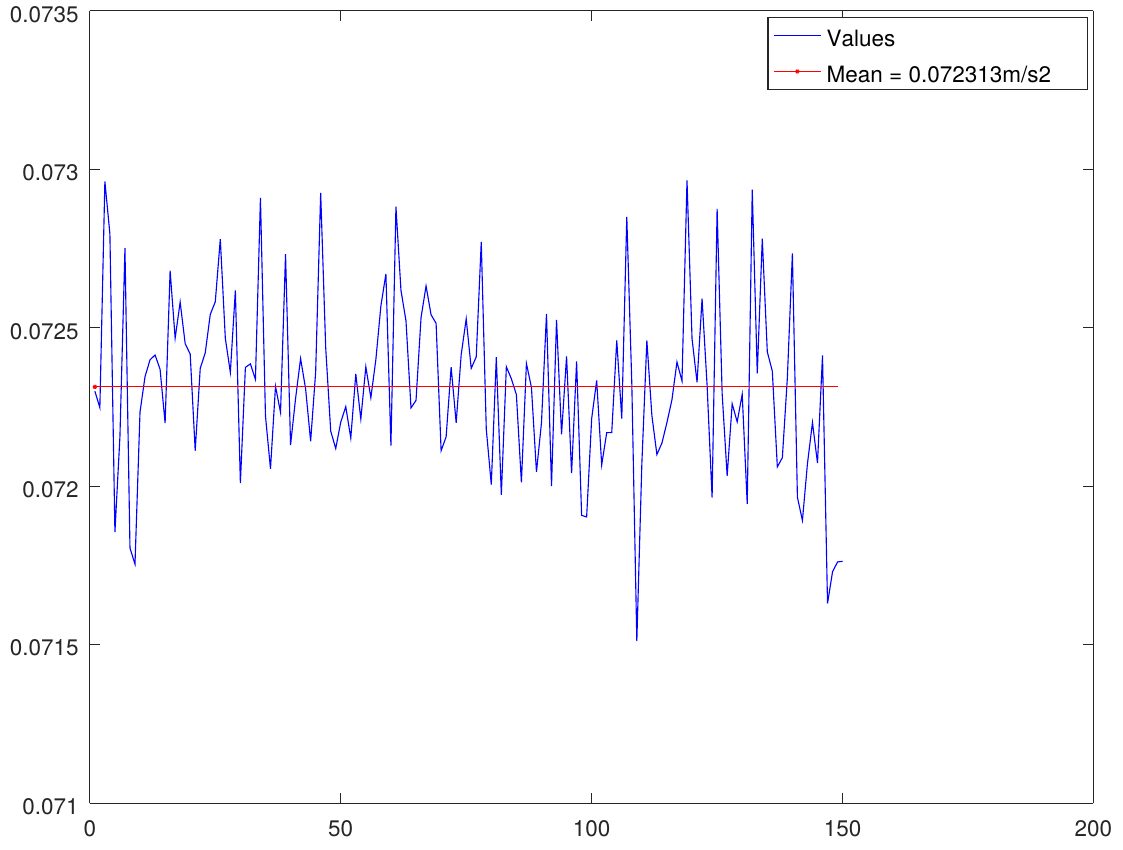
\includegraphics[width=0.7\linewidth]{valuesPlot.png}
\caption*{\texttt{Valori osservati e media}}
\label{fig:valuesplot}
\end{figure}\newpage
\texttt{Istogrammi con bin di lunghezza fissa:}
\begin{figure}[h]
	\centering
	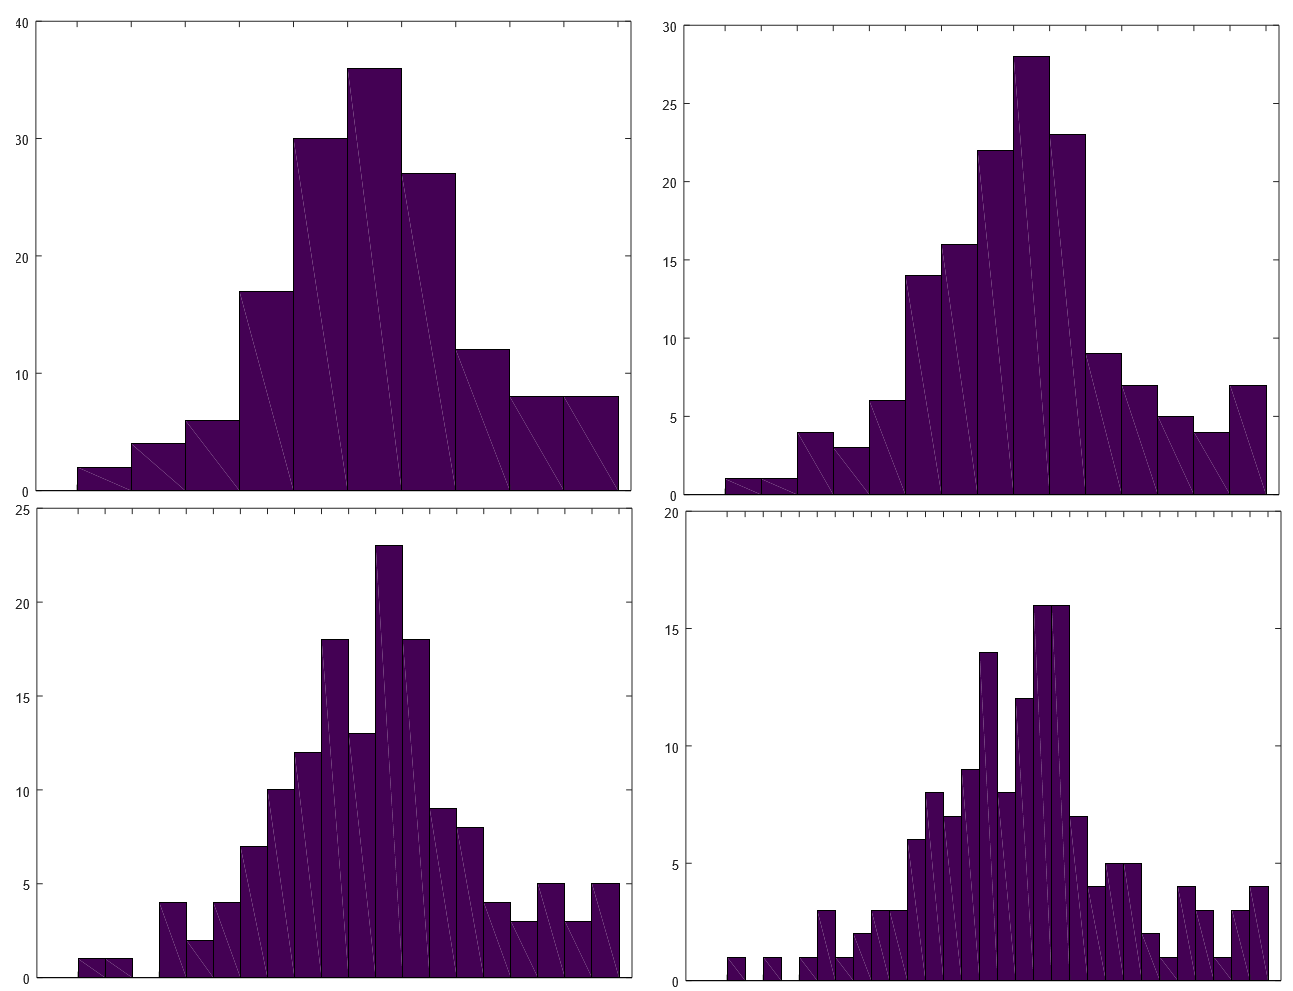
\includegraphics[width=0.7\linewidth]{hist}
	\caption*{\texttt{Numero di bin = 10, 15, 20, 30}}
	\label{fig:hist}
\end{figure}\\*
\texttt{Istogrammi con bin di lunghezza variabile:}
\begin{figure}[h]
	\centering
	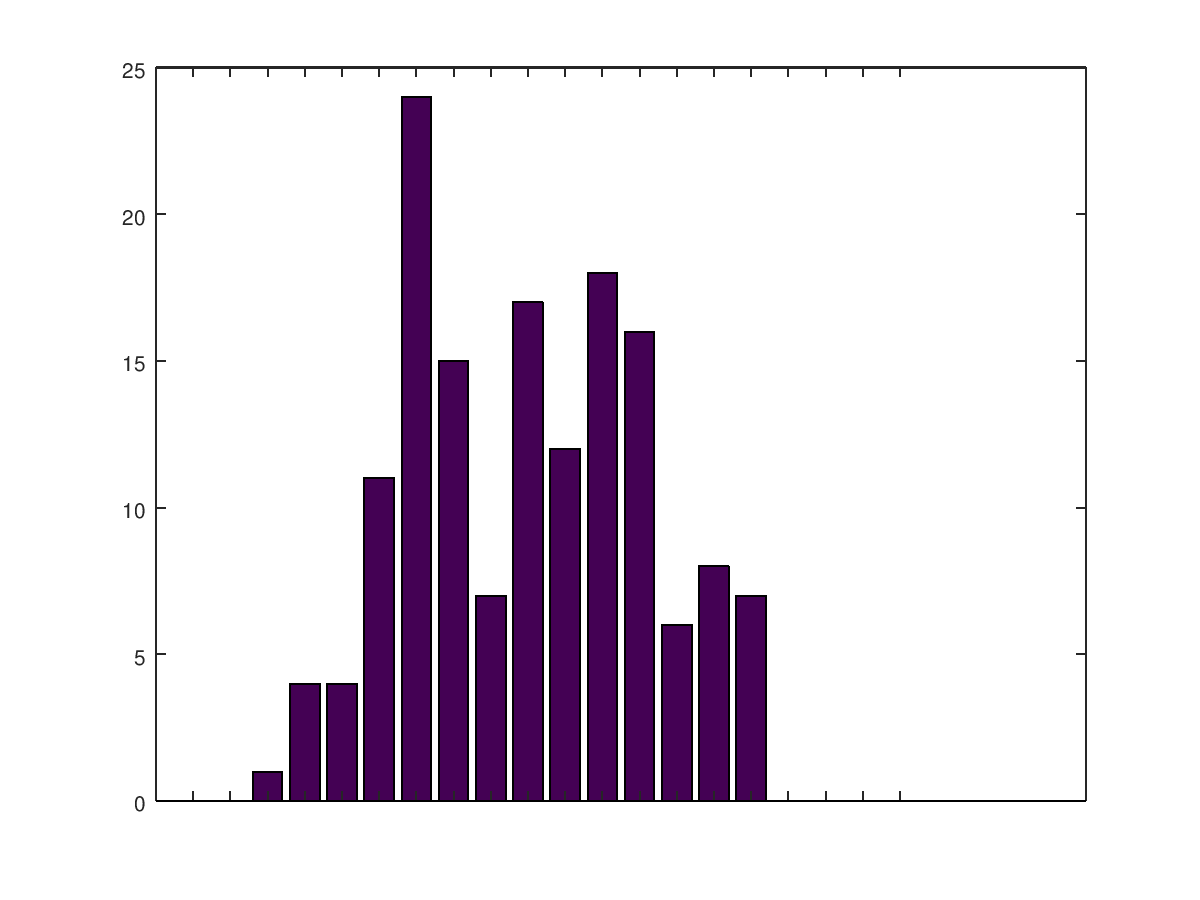
\includegraphics[width=0.7\linewidth,height=0.4\linewidth]{barsNonFixedBinspace}
	\caption*{\texttt{ $[\mu\pm$4$\sigma$,$\mu\pm$3.5$\sigma$,$\mu\pm$3$\sigma$,$\mu\pm$2.5$\sigma$,$\mu\pm$2$\sigma$,$\mu\pm$1.5$\sigma$,$\mu\pm\sigma$,$\mu\pm\frac{\sigma}{2}$,$\mu\pm\frac{\sigma}{4}$,$\mu\pm\frac{\sigma}{8}]$}}
	\label{fig:bar}
\end{figure}\\*
\texttt{Frequenze osservate:}
\begin{center}
\begin{tabular}{|c|c|c|}
	\hline 
	\texttt{Intervallo} & \texttt{Frequenza assoluta} & \texttt{Frequenza relativa} \\ 
	\hline 
	$\mu\pm3\sigma$ & \texttt{150} & \texttt{1.00000} \\ 
	\hline 
	$\mu\pm2\sigma$ & \texttt{145} & \texttt{0.96667} \\ 
	\hline 
	$\mu\pm\sigma$ & \texttt{115} & \texttt{0.76667} \\ 
	\hline 
	$\mu\pm\frac{\sigma}{2}$ & \texttt{85} & \texttt{0.56667} \\ 
	\hline 
	$\mu\pm\frac{\sigma}{2}$ & \texttt{54} & \texttt{0.36000} \\ 
	\hline 
	$\mu\pm\frac{\sigma}{8}$ & \texttt{29} & \texttt{0.19333} \\ 
	\hline 
\end{tabular} 
\end{center}
\newpage
\mbox{}\\*
\texttt{Distribuzione limite:}
\begin{figure}[h]
	\centering
	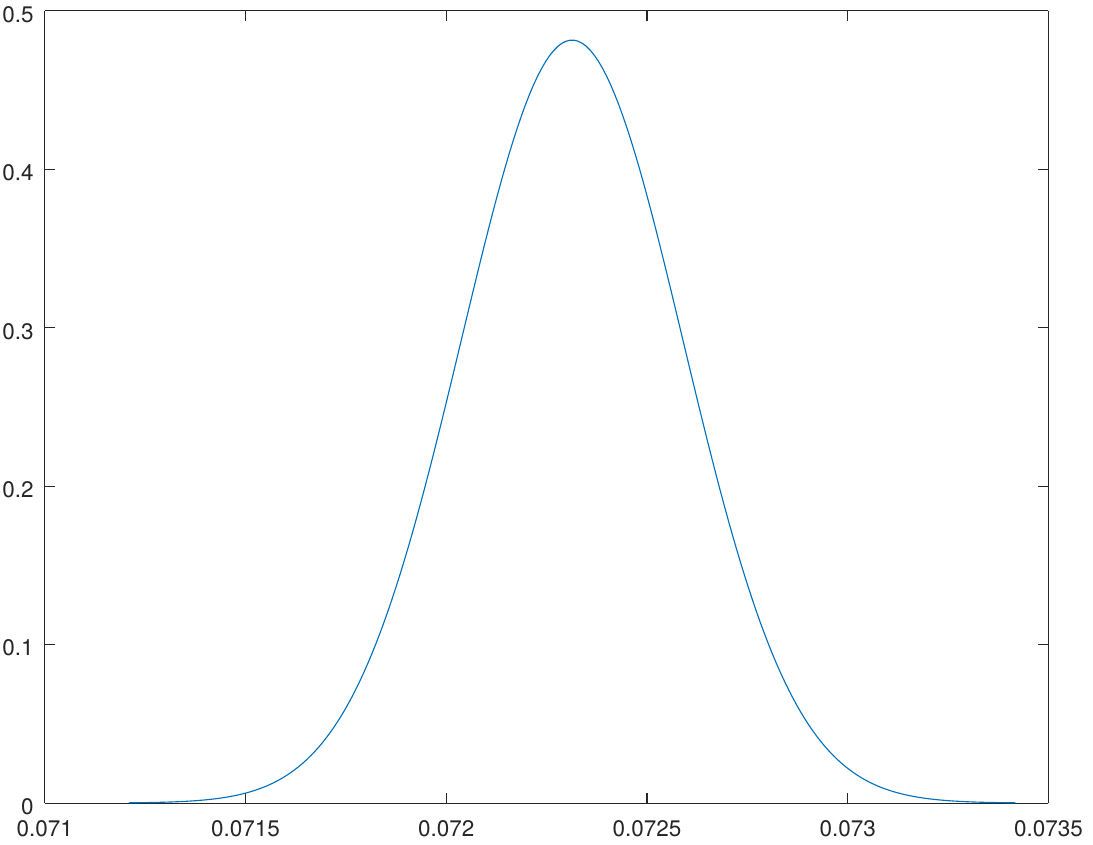
\includegraphics[width=0.7\linewidth]{limDist}
	\label{fig:limitdistribution}
\end{figure}
\begin{center}
	\begin{tabular}{|c|c|c|}
		\hline 
		\texttt{Intervallo} & \texttt{Probabilit�} \\ 
		\hline 
		$\mu\pm3\sigma$ & $1-P(X<3\sigma) - P(x>3\sigma) = 0.9737$ \\ 
		\hline 
		$\mu\pm2\sigma$ & $1-P(X<2\sigma) - P(x>2\sigma) = 0.9523$ \\ 
		\hline 
		$\mu\pm\sigma$ & $1-P(X<\sigma) - P(x>\sigma) = 0.6827$ \\ 
		\hline 
		$\mu\pm\frac{\sigma}{2}$ & $1-P(X<\frac{\sigma}{2}) - P(x>\frac{\sigma}{2}) = 0.3829$ \\ 
		\hline 
		$\mu\pm\frac{\sigma}{4}$ & $1-P(X<\frac{\sigma}{4}) - P(x>\frac{\sigma}{4}) = 0.1974$ \\ 
		\hline 
		$\mu\pm\frac{\sigma}{8}$ & $1-P(X<\frac{\sigma}{8}) - P(x>\frac{\sigma}{8}) = 0.0995$  \\ 
		\hline 
	\end{tabular} 
\end{center}

\end{document}